\documentclass[a4paper,12pt]{article}
\usepackage{graphicx}
\usepackage{geometry}
\geometry{margin=0.9in}

\begin{document}

% ================= PAGE 1 =================

\begin{center}

\includegraphics[width=0.25\textwidth]{iiitb_comet_logo.jpg}

\vspace{0.3cm}

{\huge \textbf{ARM Task Implementation}}

\vspace{0.3cm}

\textbf{Name: Srinidhi A} \\
\textbf{ID: COMETFWC053}
\end{center}

\vspace{0.6cm}

\section*{Question 36 (GATE EC 2009)}

If $X = 1$ in the logic equation

\begin{center}
$F = [X + Z(Y + (Z + XY)')][(\overline{Y} + \overline{Z}(X + Y))]$
\end{center}

and $F = 1$, then the correct option is:

\begin{enumerate}
\item[(a)] $Y = Z$
\item[(b)] $Y = \overline{Z}$
\item[(c)] $Z = 1$
\item[(d)] $Z = 0$
\end{enumerate}

\section*{Detailed Solution}

Given:

$F = [X + Z(Y + (Z + XY)')][(\overline{Y} + \overline{Z}(X + Y))]$

Substitute $X = 1$:

$F = [1 + Z(Y + (Z + Y)')][(\overline{Y} + \overline{Z}(1 + Y))]$

Using Boolean identities:

$1 + A = 1$, \quad $1 + Y = 1$

Thus,

$F = \overline{Y} + \overline{Z}$

Using De Morgan’s theorem:

$F = \overline{YZ}$

\textbf{Correct Option: (a) $Y = Z$}

\newpage

% ================= PAGE 2 =================

\section*{Truth Table}

\begin{center}
\begin{tabular}{|c|c|c|}
\hline
Y & Z & $F = \overline{YZ}$ \\
\hline
0 & 0 & 1 \\
0 & 1 & 1 \\
1 & 0 & 1 \\
1 & 1 & 0 \\
\hline
\end{tabular}
\end{center}

\vspace{0.5cm}

\section*{Gate Diagram Representation}

\begin{center}
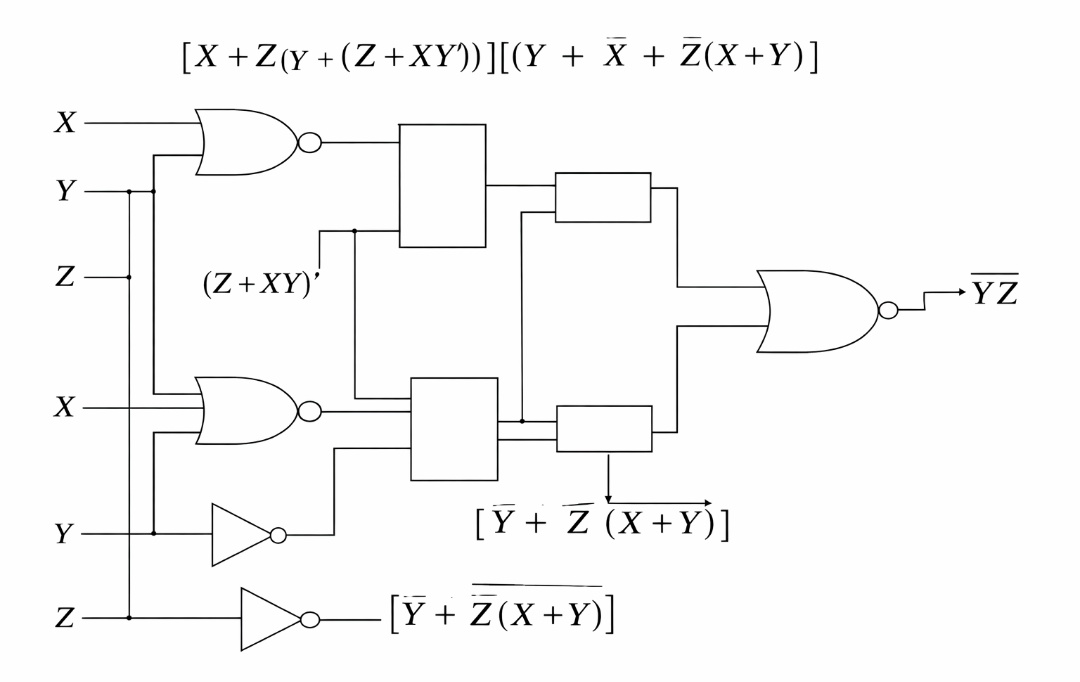
\includegraphics[width=0.75\textwidth]{gate_diagram.jpg}
\end{center}

Simplified implementation: 2-input NAND Gate.

\newpage

% ================= PAGE 3 =================

\section*{Hardware Implementation}

\begin{center}

\includegraphics[width=0.6\textwidth]{hardware.jpg}
\end{center}

\section*{Steps to Perform the Task}

\begin{enumerate}
\item Connect switch Y to GPIO14 (pull-up).
\item Connect switch Z to GPIO15 (pull-up).
\item Connect LED to GPIO16 via 220$\Omega$ resistor.
\item Connect 7-segment display to GPIO pins 2–8.
\item Upload MicroPython code.
\item Toggle Y and Z switches and observe output.
\item Verify output follows NAND logic.
\end{enumerate}

\section*{Conclusion}

After simplification, the Boolean expression reduces to:

\begin{center}
$F = \overline{YZ}$
\end{center}

\end{document}

